\documentclass[12pt,a4paper]{article}
\usepackage[utf8]{vietnam}
\usepackage{amsmath}
\usepackage{amsfonts}
\usepackage{amssymb}
\usepackage{graphicx}
\usepackage[left=2.5cm,right=2.5cm,top=2cm,bottom=2cm]{geometry}
\usepackage{listings} % môi trường để ghi code
\usepackage{color} % tô màu cho code
\usepackage{blindtext}
% ------------------------ Giúp khởi tạo môi trường viết code (tự động tô màu Syntax)
\definecolor{dkgreen}{rgb}{0,0.6,0}
\definecolor{gray}{rgb}{0.5,0.5,0.5}
\definecolor{mauve}{rgb}{0.58,0,0.82}
\lstset{frame=tb,
  language=C,
  aboveskip=3mm,
  belowskip=3mm,
  showstringspaces=false,
  columns=flexible,
  basicstyle={\small\ttfamily},
  numbers=none,
  numberstyle=\tiny\color{gray},
  keywordstyle=\color{blue},
  commentstyle=\color{dkgreen},
  stringstyle=\color{mauve},
  breaklines=true,
  breakatwhitespace=true,
  tabsize=3
}
%----------------------------
\renewcommand{\baselinestretch}{1.3} % lệnh này cho phép điều chỉnh khoảng cách chung giữa CÁC DÒNG
\setlength{\parskip}{1em} % Lệnh này điều chỉnh khoảng cách giữa CÁC ĐOẠN

\title{\textbf{C Language \& Affect}\thanks{Một bài phân tích, đánh giá và cảm nhận nhỏ trong quá trình tự học C}}
\date{2020\\ Feb}
\author{Phạm Anh Tuấn\\ \\ \textit{Posts and Telecommunications Institute of Technology} \and Km10, Đường Nguyễn Trãi, Q.Hà Đông, Hà Nội}


\begin{document}
\maketitle
\begin{center}
	\textbf{\large Tóm Tắt}
\end{center}


Ngôn ngữ C lần đầu được thiết kế bởi Dennis Ritchie tại phòng thí nghiệm Bell Telephone năm 1972. Được phát triển dựa theo ngôn ngữ B nhằm mục đích chính là xây dựng hệ điều hành UNIX. Chính vì thế nó không đem lại sự tiện dụng cho người lập trình. Nhưng C là ngôn ngữ \textbf{mạnh} và \textbf{linh hoạt} nên nhanh chóng trở thành ngôn ngữ phổ biên được lập trình viên viết nhiều loại ứng dụng ở các mức độ khác nhau. Ngày nay có nhiều ngôn ngữ lập trình mạnh mẽ và tính ứng dụng cao hơn, tuy nhiên nhờ những đặc tính nổi bật của nó nên C là lựa chọn tốt trong việc học và sau này là lập trình hướng đối tượng nơi mà ngôn ngữ C++ hỗ trợ rất nhiều mà C làm nền tảng.
\newpage
\section{Các vấn đề sơ khai}
\subsection{Biến, Hằng và Các kiểu dữ liệu liên quan }
 Đối với những người mới bắt đầu thì lập trình trên Console Window có thể coi là bước nhập môn bắt buộc. Bỏ qua GUI\footnote{Giao diện đồ họa người dùng, được sử dụng khá rộng rãi trong ngành CNTT hiện nay. Đây như là một cách giao tiếp với máy tính bằng hình ảnh và chữ viết thay vì các dòng lệnh đơn thuần, giúp đưa ra những trải nghiệm trực quan}, làm việc trên Console đưa cho ta góc nhìn về bản chất nhất. Và những "Nhân vật " chủ chốt phải kể đến là \textbf{Biến} . 

\textbf{Biến} rất dễ hiểu như là "cái hộp" dùng để chứa những dữ liệu. Khác với biến x,y,z... trong toán học. Những chiếc hộp này được xác định ở một vị trí mà máy tính tự dộng chỉ thị. \textbf{Hằng} là một loại giống biến, chỉ khác dữ liệu \& địa chỉ của nó được bạn khai báo và xác định trước. Nói cách khác, đây là một cái hộp không trống

Và trong lập trình, ta luôn tập trung đến việc "Làm ít, hiệu quả tối ưu". Môi trường lập trình mà ta làm việc không thể như vũ trụ luôn giãn nở được, để tránh lượng dư thừa không cần thiết thì những cái hộp chứa dữ liệu ấy không được quá lớn hay quá nhỏ so với dữ liệu mà nó phải chứa. Định nghĩa kiểu dữ liệu cho kích thước biến cũng hình thành ra
\begin{center}
\begin{itemize}
	\item Kiểu số nguyên
\begin{center}
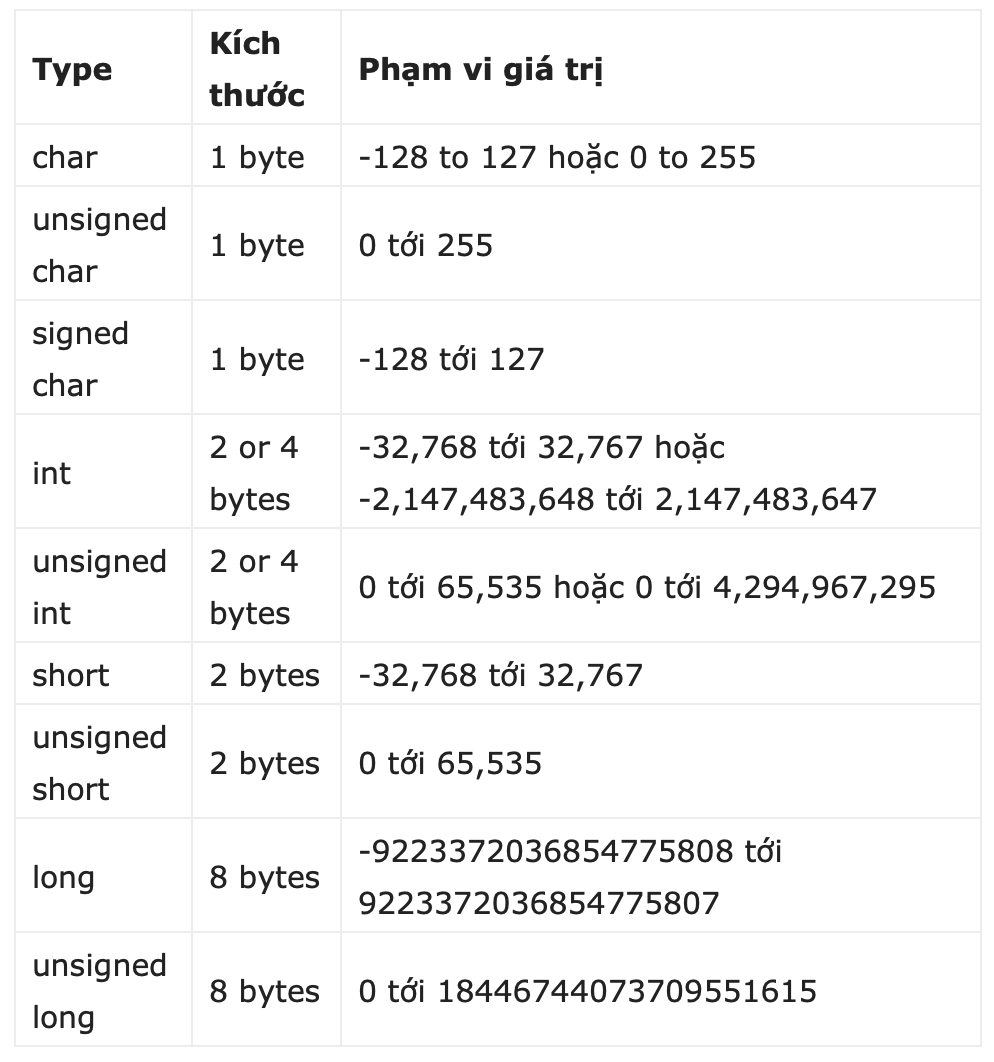
\includegraphics[scale=0.55]{kieusonguyen.png}
\end{center}
	\item Kiểu số nguyên
\begin{center}
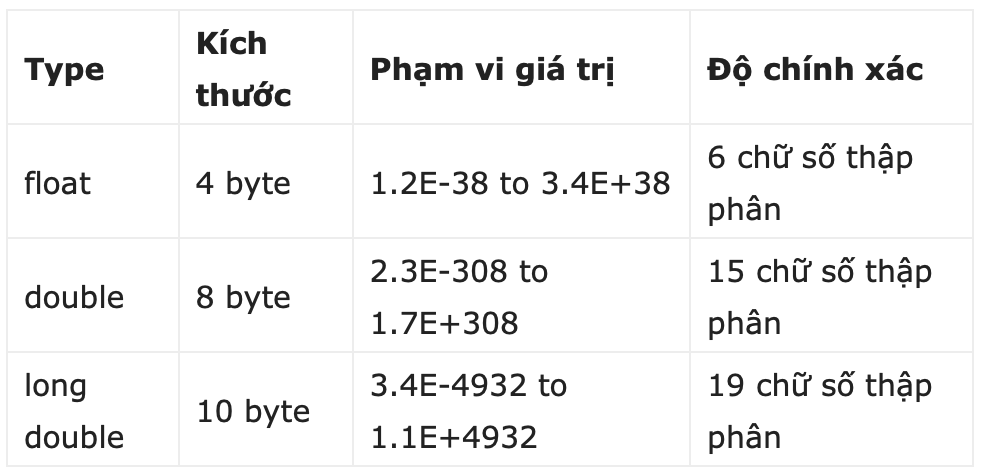
\includegraphics[scale=0.7]{kieusothuc}
\end{center}

\item Kiểu ký tự 
\begin{center}
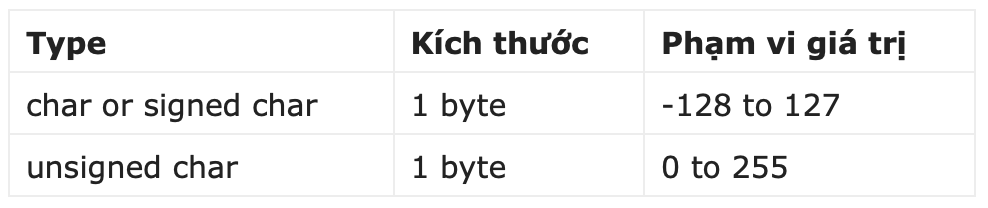
\includegraphics[scale = 0.7]{kieukytu}
\end{center}
\end{itemize}	
\end{center}

\subsection{Nhập \& Xuất - Nơi khiến dữ liệu được tổ chức và trực quan hoá}

\begin{itemize}
	\item Hàm nhập 'scanf()':
	 \begin{itemize}
            \item Được dùng để đọc các kiểu dữ liệu mà người dùng nhập từ bàn phím.             
            \item Hàm 'scanf()' nhận vào tham số là \textbf{địa chỉ} của biến chứ không đơn thuần là giá trị của biến. Thế nên có hai thành phần mà ta nên chú ý là địa chỉ và giá trị khi dùng hàm 'scanf()
            \item Cấu trúc cơ bản: scanf("<Kiểu giả trị biến>", \&<Tên biến>)\footnote{Dấu '\&' trong hàm scanf() dùng để chỉ địa chỉ của biến };
     \end{itemize}
	 \item Hàm xuất 'printf()':
	\begin{itemize}
            \item Dùng để in ra các ký tự, chuỗi ... hiển thị lên màn hình console.
            \item Cấu trúc cơ bản của hàm printf("Tên bạn muốn hiển thị trên cửa sổ + \%<kiểu dự liệu bạn muốn trích ra từ biến>",<tên gọi các biến được truyền vào> ....)
            \item Các ký tự biểu thị các định dạng kiểu dữ liệu:\\ 
           	\begin{center}
           	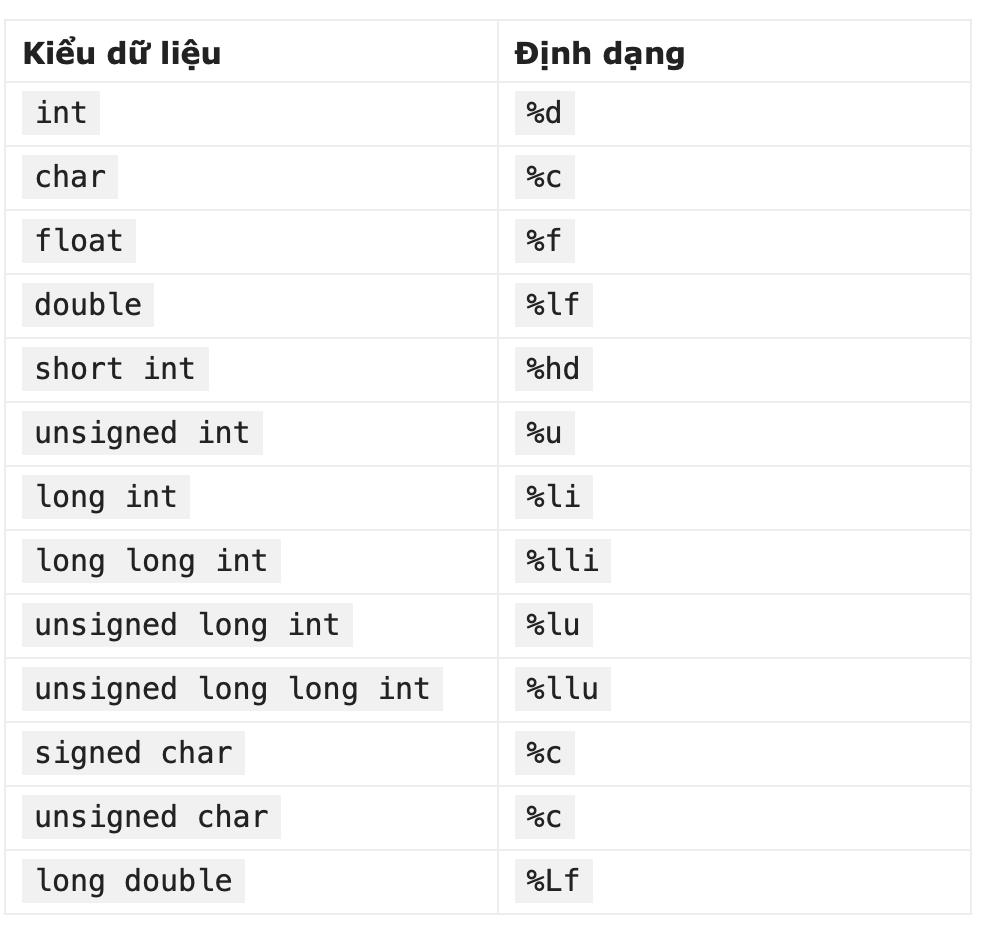
\includegraphics[scale = 0.6]{kieudulieu}	
           	\end{center}
     \end{itemize}
\end{itemize}

\subsection{Toán tử}

Một loạt các phép tính mà máy tính dùng để tác động \textbf{trực tiếp} lên các biến. Nó khá giống các phép toán thông thường nhưng được bổ xung thêm một số toán tử đặc trưng trong lập trình
\subsubsection{Toán tử số học (Arithmetic Operators)}
Còn được gọi là \textbf{toán tử 2 ngôi} khi nó được dùng để tham gia các phép toán với sự tham gia của 2 giá trị
\begin{center}
	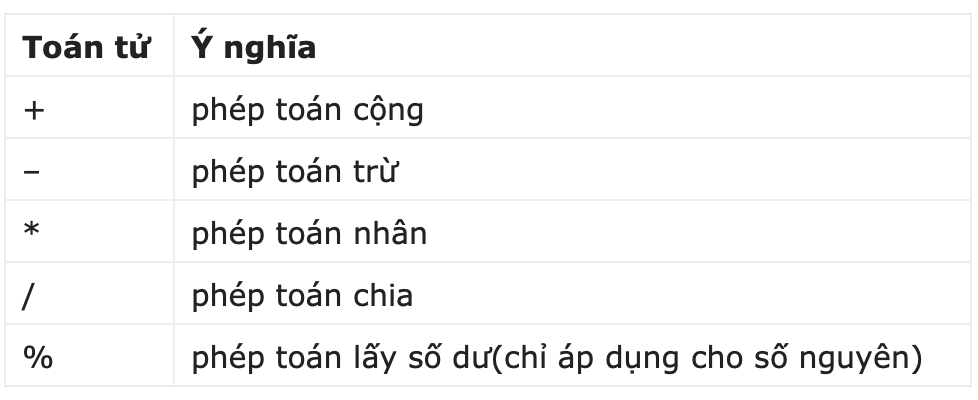
\includegraphics[scale =0.7]{ArithmeticOperators}
\end{center}
\subsubsection{Toán tử tăng giảm}
\begin{itemize}
	\item Toán tử '++': Tăng giá trị biến lên 1 đơn vị
	\item Toán tử '--': Giảm giá trị biến đi 1 đơn vị
\end{itemize}
\subsubsection{Toán tử gán (Assignment Operators)}
Để gán giá trị của 1 biến trong lập trình 
\begin{center}
	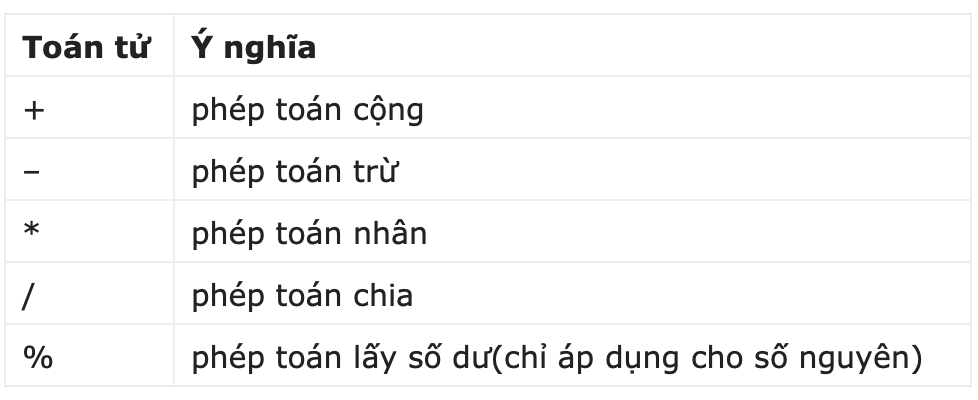
\includegraphics[scale =0.7]{ArithmeticOperators}
\end{center}
\subsubsection{Toán tử quan hệ (Relational Operators)}
Dùng để \textbf{kiểm tra} mối quan hệ giữa các toán hạng từ đó trả về giá trị 'TRUE' hoặc 'FALSE'
\begin{center}
	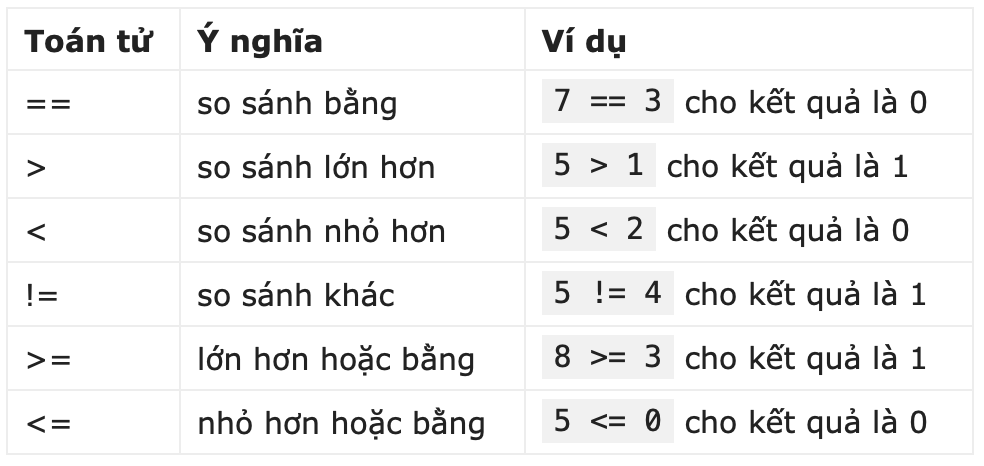
\includegraphics[scale =0.7]{RelationalOperators}
\end{center}
\subsubsection{Toán tử Logic (Logical Operators)}
Gồm những toán tử với các công dụng sau:
\begin{itemize}
	\item Toán tử '\&\&': là toán tử AND, trả về 'TRUE' khi và chỉ khi tất cả các toán hạng đều đúng.
	\item Toán tử '||': là toán tử OR, trả về 'TRUE' khi có ít nhất 1 toán hạng đúng.
	\item Toán tử '!': là toán tử NOT, phủ định giá trị của toán hạng.
\end{itemize}
\subsubsection{Các toán tử khác }
\begin{itemize}
	\item Toán tử Bit
	\item Toán tử Comma Operator
	\item Toán tử sizeof Operator
\end{itemize}
\section{Cấu trúc điều khuyển}
Cấu trúc điều khuyển hiểu đơn giản là tập các câu lệnh giúp điều phối luồng chạy dữ liệu và xử lý dữ liệu biến trong lập trình bên cạnh các yếu tố then chốt khác như: Hàm, Mảng, Chuỗi và Con trỏ ... Để dễ hình dung và đỡ lẫn lộn giữa cấu trúc điều khuyển nói chung hay các câu lệnh nói riêng với toán tử là "\textbf{Câu Lệnh} có thể biểu diễn dưới dạng lưu đồ thuật toán còn \textbf{Toán Tử} là cách xử lý có trong lưu đồ thuật toán."
\begin{center}
\section*{Rẽ nhánh}	
\end{center}
\subsection{Cấu lệnh điều khuyển If }
Là thành phần được sử dụng gần như trong mọi chương trình phần mềm, thế nên việc nắm rõ được khối điều khuyển này sẽ giúp bạn làm chủ chương trình.

	Câu lệnh có cấu trúc và lưu đồ thuật toán được biểu diễn như sau:
%Ghi code ở đây
\begin{lstlisting}
if (<Dieu kien>){
    // Khoi lenh se duoc thuc hien neu <Dieu Kien> dung
}\end{lstlisting}
%--------------
\begin{center}
	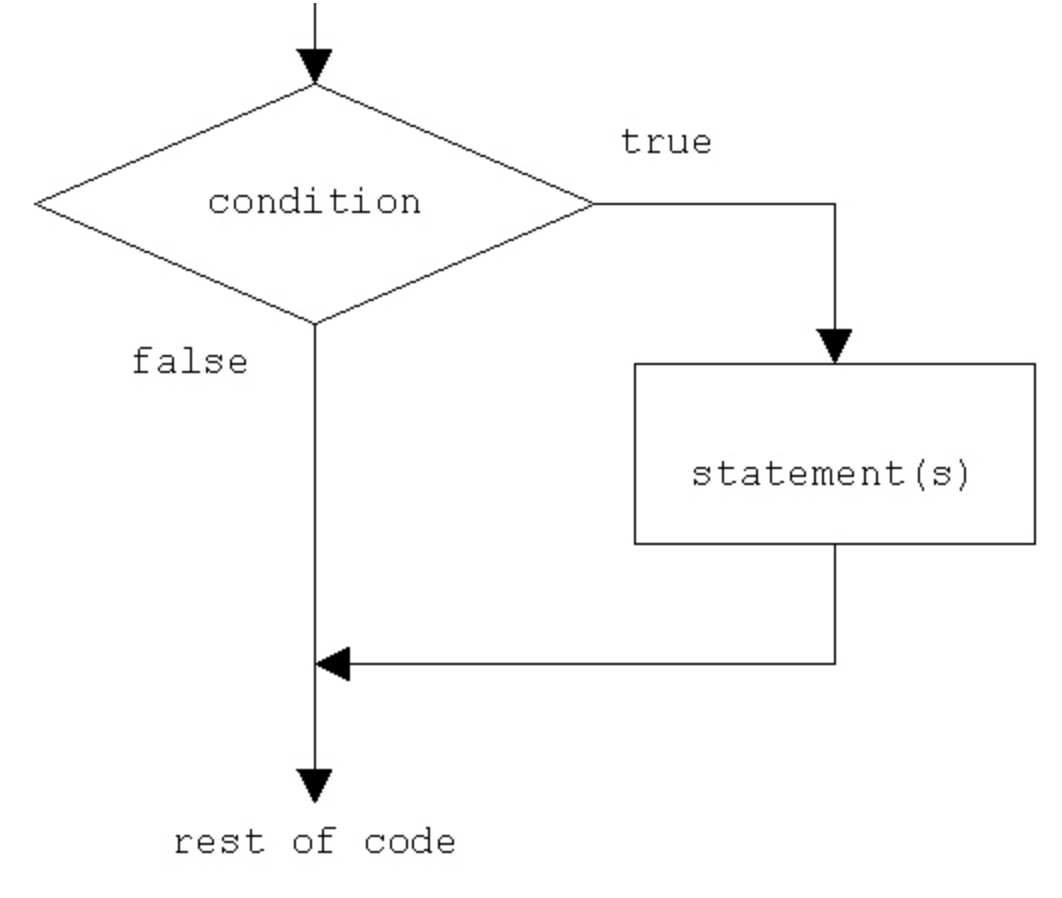
\includegraphics[scale = 0.7]{Ifelsestatement}
\end{center}

\subsection{Câu lệnh điều khuyển If ... Else}
Câu lệnh và lưu đồ thuật toán\footnote{Lưu đồ thuật toán (Flow Chart): là một sơ đồ có các khối và các đường dẫn chỉ định} của khối lệnh này
\begin{lstlisting}
if (<Dieu kien>){
   <khoi lenh se thuc hien dieu kien dung>
}else {
	<Khoi lenh se thuc hien ney dieu kien sai>
}
\end{lstlisting}
\begin{center}
	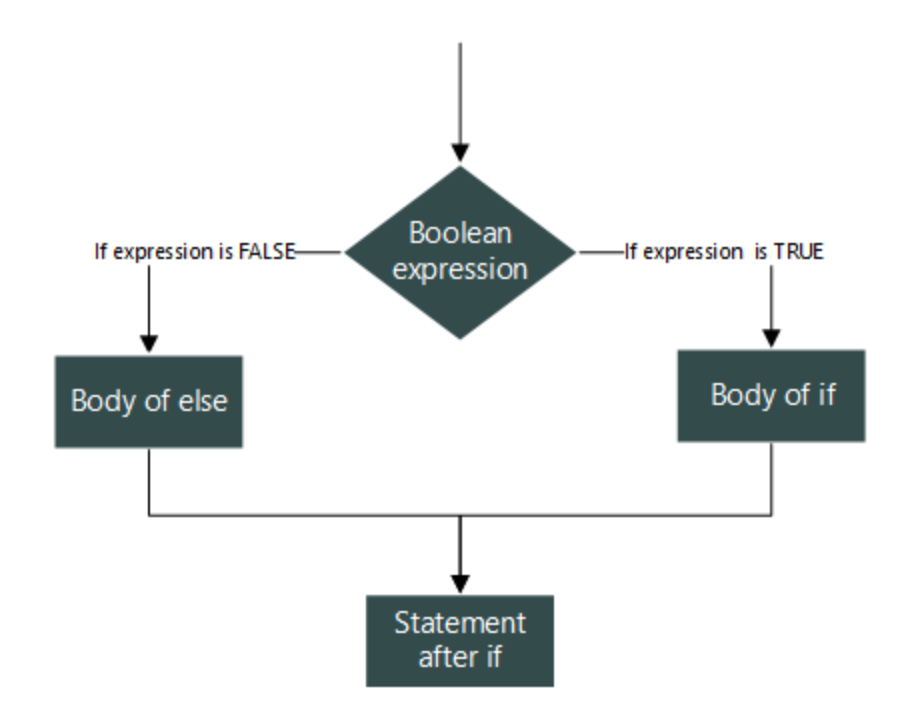
\includegraphics[scale =0.45]{caulenhifelse}
\end{center}

\subsection{Cấu lệnh điều khuyển Switch - Case}
Tương tự về cấu trúc như If-else tuy nhiên việc sử dụng Switch-case đem lại khả năng dễ viết và đọc hơn. Nếu để ý kĩ hơn một chút, cấu trúc If-else mang xu hướng “Lọc” dữ liệu lớn đầu vào trong hầu hết các bài toán còn cấu trúc \textbf{Switch} mang tính lựa chọn, dựa vào yêu cầu người dùng nhập vào nhiều hơn từ đó xử lý bài toán theo các hàm mà người dùng đã định nghĩa trước (giống như việc ta sử dụng máy tính cầm tay để nó tính toán các số vậy).

\begin{lstlisting}

switch (expression){
    case constant1:
      // statements
      break;
    case constant2:
      // statements
      break;
    . . .
    default:
      // default statements
}
\end{lstlisting}
\begin{center}
	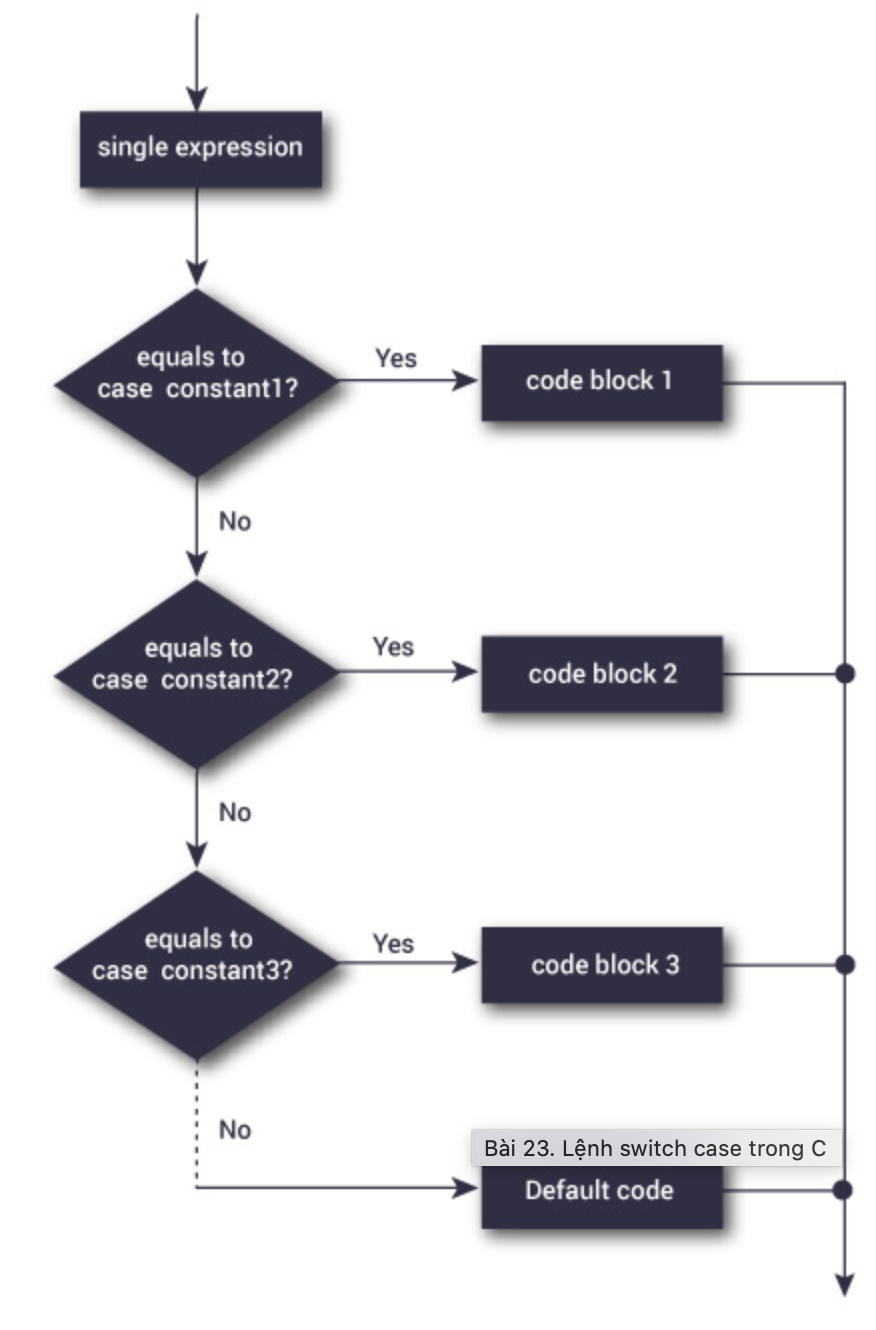
\includegraphics[scale = 0.45]{Switchcaseflowchart}
\end{center}

\begin{center}
\section*{Vòng lặp}	
\end{center}


Tương tự như cấu trúc rẽ nhánh, vòng lặp được sử dụng khá nhiều trong việc xây dựng và phát triển phần mềm. Đặc trưng của \textbf{vòng lặp } là giúp chúng ta giải quyết các công việc lặp lại chỉ bằng những dòng code rất gọn
\subsection{Vòng lặp For}
Câu lệnh và lưu đồ thuật toán 
\begin{lstlisting}
for(<khoi tao gia tri bien lap>;<Dieu kien lap>;<cap nhat bien>){
	<khoi lenh>
}
\end{lstlisting}
\begin{center}
	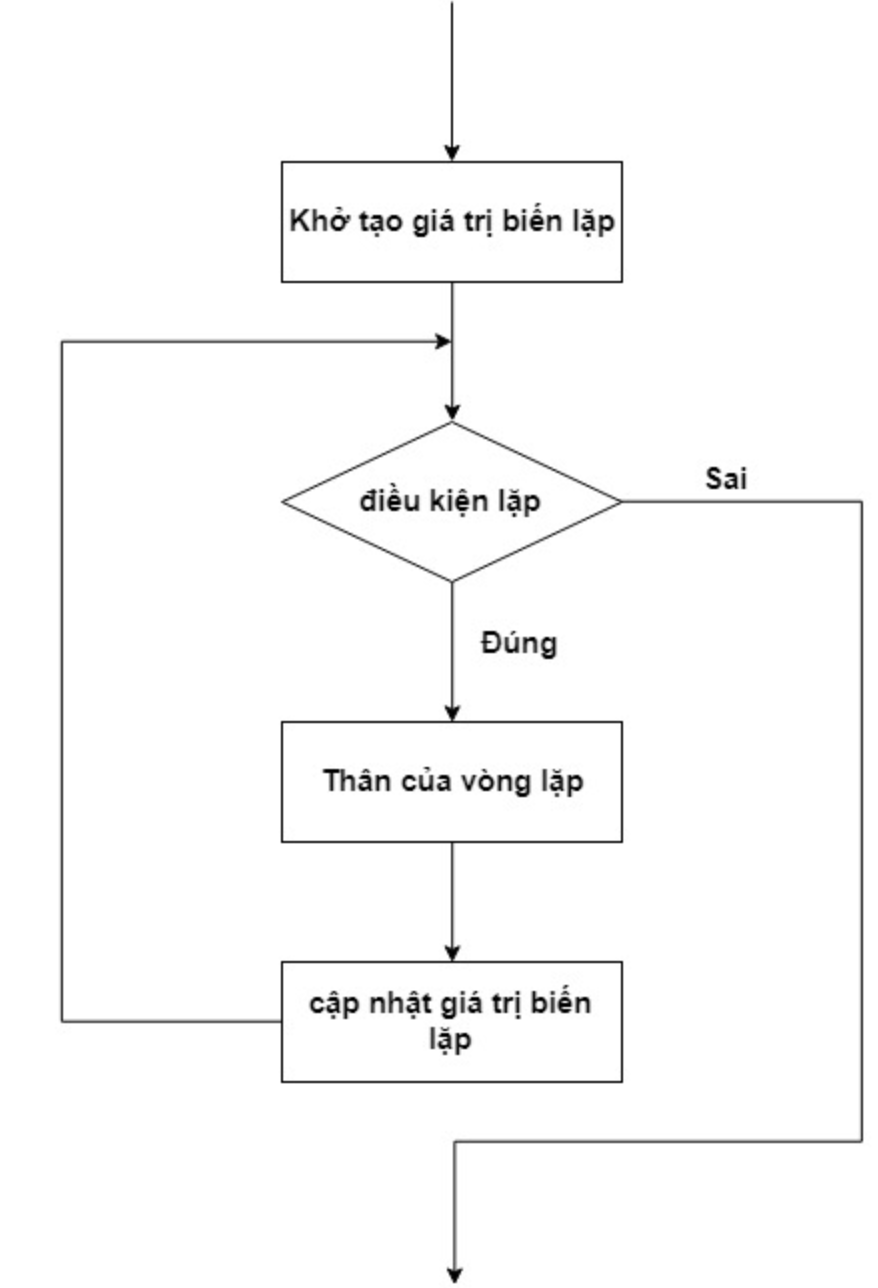
\includegraphics[scale = 0.7]{forflowchart}
\end{center}
\subsection{Vòng lặp While / Do ... While}
Tương tự như vòng lặp For về điều hướng cấu trúc lệnh, tuy nhiên vòng lặp While/Do..While rất thích hợp cho việc lặp mà số lần không biết trước hay không xác định được. Điểm này thật sự cần lưu ý bởi nếu không cẩn thận sẽ dễ bị vòng lặp vô tận nếu điều kiện bên trong câu lệnh lặp không hợp lý
\begin{itemize}
	\item Vòng lặp \textbf{While}: \\
Đặc điểm của vòng lặp này là điều kiện được kiểm tra trước rồi mới khởi chạy câu lệnh
 \begin{lstlisting}
while (testExpression){
    // statements inside the body of the loop 
}
\end{lstlisting}

\begin{center}
	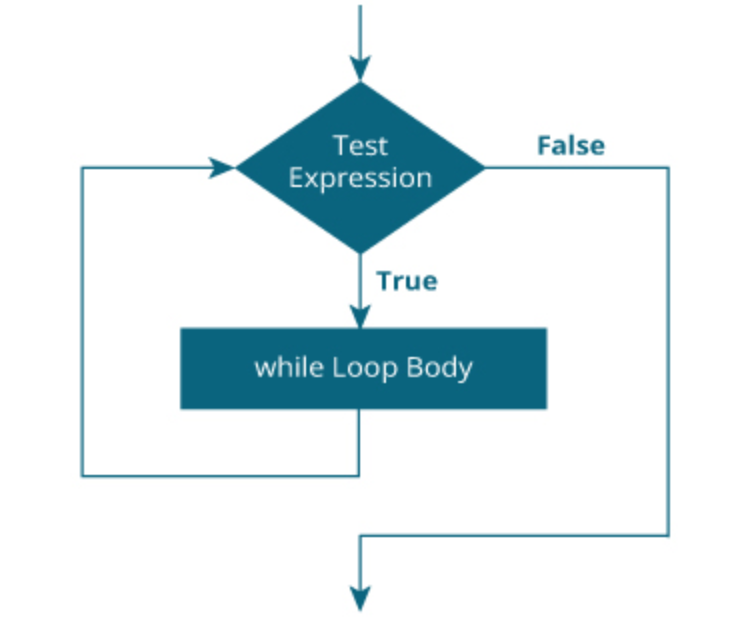
\includegraphics[scale =1]{whileflowchart}
\end{center}
\item Vòng lặp \textbf{Do..While} \\
Đặc điểm của vòng lặp này là câu lệnh được thực thi trước khi điều kiện được kiểm tra.
\begin{lstlisting}
	do{
	... <khoi lenh>
	}whlie(<dieu kien vong lap>)
\end{lstlisting}
\begin{center}
	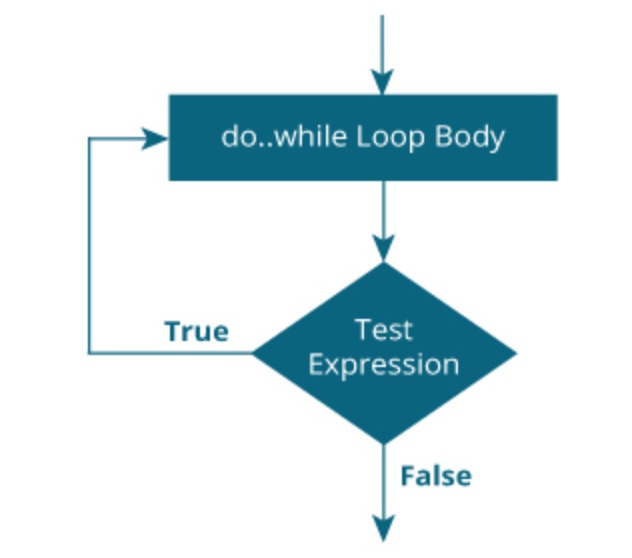
\includegraphics[scale = 1]{dowhileflowchart.png}
\end{center}
\end{itemize}
\begin{center}
\section*{Lệnh Break \& Continue \footnote{Đây là những lệnh kiểm soát vòng lặp}}		
\end{center}
Việc sử dung những lệnh này cho phép chúng ta quản lý và làm việc với vòng lặp hiệu quả hơn. Đặc điểm của những câu lệnh này là nó thường xuất hiện khi được “bao bọc” bởi khối lệnh "if" bởi nếu không có lệnh "if" thì vòng lặp trở nên vô dụng
\begin{itemize}
	\item Lệnh Break:\\
Về cơ bản một vòng lặp khi thực thi nếu gặp lệnh break sẽ thoát vòng lặp ngay lập tức. Sơ đồ mô tả hoạt động
	\begin{center}
		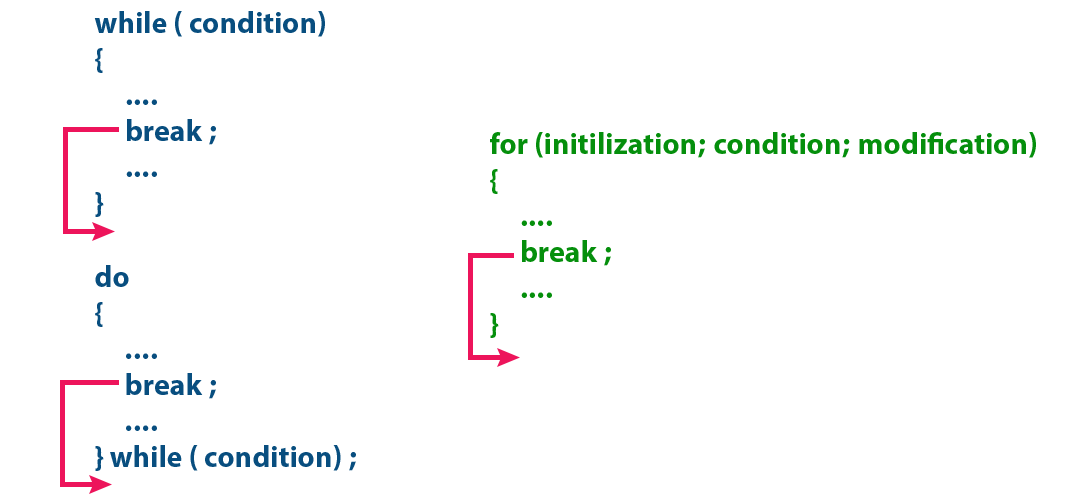
\includegraphics[scale = 0.4]{break}
	\end{center}

\begin{lstlisting}
	#include <stdio.h>
 
int main(){
    int number;
    printf("\nNhap number = ");
    scanf("%d", &number);
 
    bool allEven = true; // gia su ban dau la dung
    int last;
    while(number > 0){
        last = number % 10; // Lay chu so cuoi cua number
 
        if(last % 2 == 1){
            allEven = false;
            break; // thoat vong lap
        }
        number /= 10; // bo chu so cuoi cua Number
    }
    
    if(allEven){
        printf("\nToan chu so chan!");
    }else{
        printf("\nCo chu so le!");
    }
 
}
\end{lstlisting}
	\item Lệnh Continue:\\
Một vòng lặp đang chạy mà gặp lệnh \textbf{"continue"}, tất cả các lệnh trong thân vòng lặp nằm phía dưới lệnh \textbf{"continue"} sẽ bị bỏ qua ở lần lặp hiện tại chuyển qua điều kiện và tiếp tục lặp (Nếu điều kiện lặp còn thoả mãn). Sơ đồ mô tả hoạt động:
\begin{center}
	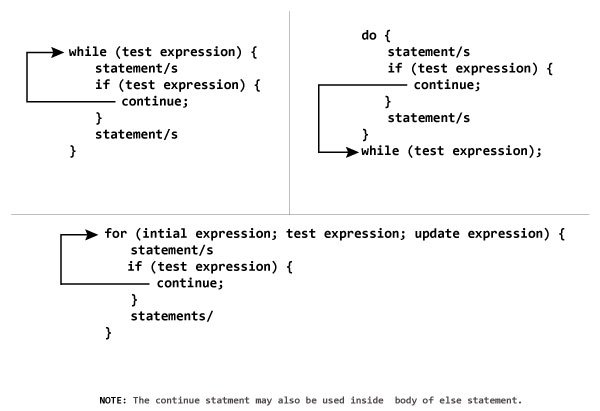
\includegraphics[scale =0.7]{lenhcontinue}
\end{center}
\end{itemize}
\section{Hàm \footnote{Bản chất thư viện khi ta đưa vào cũng là loại hàm được xây dựng sẵn. Như thư viện stdio.h chứa các hàm vào ra chuẩn }}
 \textbf{Vẻ đẹp} cũng như tính \textbf{quản lý} là điều tuyệt vời trong lập trình. Điều này luôn được ưu tiên khi mà bạn luôn phải làm việc với hàng trăm hay hàng nghìn dòng Code nên rất khó để kiểm soát cũng như tìm và sửa lỗi nếu cứ gõ lệnh tràn lan. Hàm trong C được ra đời với mục đích giải quyết vấn đề đó, tương tự như trong công ty, luôn có những phân ban với những mục đích cụ thể, giúp toàn bộ hệ thống hoạt động trơn chu. Khái quát chung về cách hoạt động của hàm: 
\begin{center}
	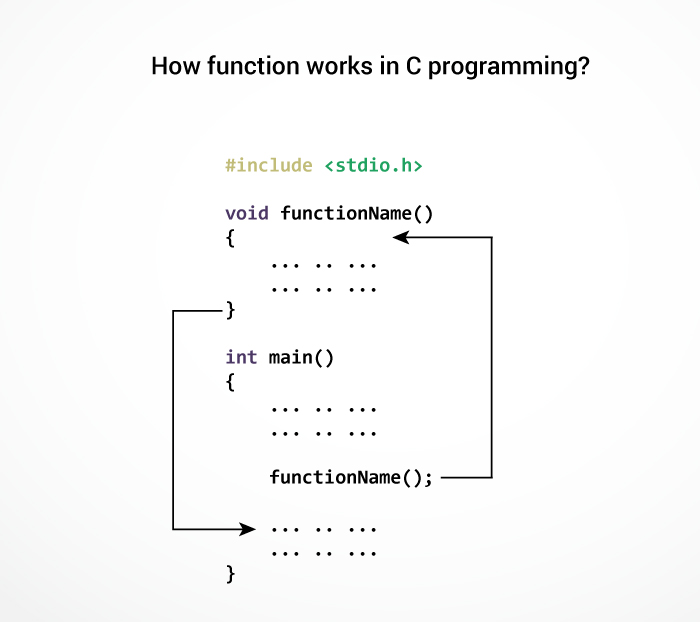
\includegraphics[scale = 0.4]{functionwork}
\end{center}
\begin{center}
\subsection*{\textit{Phân loại các loại hàm}} 	
\end{center}

\subsection{Hàm không tham số đầu vào \& Không có giá trị trả về (Void)}
\subsection{Hàm có tham số \& Không có giá trị trả về (Void)}
\subsection{Hàm không tham số \& Có giá trị trả về}
\subsection{Hàm có tham số \& Có giá trị trả về}

\begin{center}
\subsection*{\textit{Hàm đệ quy}} 	
\end{center}
Một hàm khi bản thân nó tự gọi lại chính nó thì được gọi là hàm đệ quy. Ví dụ mẫu về cách hoạt động hàm đệ quy
\begin{lstlisting}
void recurse(){
		. . .
		recurse();
		. . .
}
int main()
\end{lstlisting}
Xem xét qua câu lệnh trên ta có thể thấy hàm đệ quy mang tính lặp như các cấu trúc for / while đã đề cập trước đó. Điều đó đồng nghĩa với việc phải để ý đến điều kiện để thoát vòng lặp, nếu không vòng lặp vô tận sẽ dễ xảy ra và bạn chắc chắn không muốn điều này

\begin{center}
\subsection*{\textit{Phạm vi của biến}} 	
\end{center}
Cũng là một phần nội dung con liên quan đến \textbf{hàm}. Như đã đề cập từ nội dung trước, biến là một phần khá quan trọng trong việc giải các bài toán lập trình hay nói đúng hơn lập trình hầu như chỉ có ý nghĩa khi ta làm việc với biến. Các loại biến có giá trị và phạm vi sử dụng ở môi trường hay hàm khác nhau đối với từng loại ...
\begin{itemize}
	\item Biến cục bộ (Global Variable)\\
Biến cục bộ chỉ tồn tại và chỉ có thể sử dụng bên trong khối code đó trong khi khối code đó đang thực thi đồng nghĩa là ta không dùng biến đó bên ngoài khối code được . \\Khối code được hiểu là thân 1 hàm: Hàm main() hoặc hàm con, than vòng lặp, cấu trúc If .. Elsse ....
	\item Biến toàn cục (Local Variable)\\
Trái ngược lại hoàn toàn với biến cục bộ là biến toàn cục. Chúng ta khai báo biến này ngoài tất cả các hàm và cũng sử dụng biến đó ở mọi nơi trong chương trình: Hàm main(), hàm con, câu lệnh rẽ nhánh ...
	\item Biến tĩnh (Static Variable)\\
Đặc biệt và ít dùng hơi hai biến trên là biến tĩnh. Đó là giá trị của nó luôn giữ và tồn tại cho đến hết chương trình cho dù nó là biến cục bộ hay biến toàn cục. Ta sử dụng biến tĩnh bằng các khai báo từ khoá "static", VD: static: int i;
	\item Register\\
Mang tính bên trong lõi hơn, Register được dùng đẻ khai báo các biến có tính chất cục bộ nhưng mà được lưu trong thanh ghi của CPU. Do được lưu trong thanh ghi nên việc truy xuất dữ liệu sẽ nhanh hơn so với biến được lưu trong bộ nhớ. Tuy nhiên việc khởi tạo và sử dụng biến này chỉ thật sự cần thiết nếu bạn làm việc với hệ thống nhúng hay tối ưu hoá hệ thống 
\end{itemize}
\begin{center}
	\subsection*{\textit{Tham chiếu \& Tham trị}}
\end{center}
Tham chiếu và tham trị là hai đặc tính hay trong lập trình C, để hiểu rõ hơn về cách thức hoạt động thì chúng ta sẽ đề cập đến ở phần con trỏ.
\begin{itemize}
	\item Tham trị\\
Khi ta gọi \textbf{tham trị}, việc tác động vào biến \textbf{tham trị} sẽ không ảnh hưởng tới biến ban đầu. Biến được tạo bởi tham trị là bản sao nhân đôi với biến ban đầu và hoàn toàn độc lập.
	\item Tham chiếu:\\
Khi ta gọi tham chiều, đơn giản biến đó là bản \textbf{"shortcut"} của biến ban đầu. Mọi sự tương tác với biến \textbf{"shortcut"} này bản chất là tương tác trực tiếp với biến gốc
\end{itemize}
\begin{center}
	\subsection*{\textit{Return \& Exit}}
\end{center}
\begin{itemize}
	\item Lệnh return\footnote{ Rất thích hợp để dùng cho hàm không trả về giá trị (Kiểu Void)}
Khi sử dụng lệnh này, chương trình sẽ thoát ra khi hàm gặp nó và tiếp tục trở lại thực thi những dòng Code sau lời gọi hàm đó (nếu có)
	\item Hàm Exit
Bản chất là câu lệnh hệ thống và phải khai báo thư viện stdlib.h nếu muốn sử dụng. Khi sử dụng hàm Exit chương trình sẽ kết thúc ngay lập tức
\end{itemize}

\section{Mảng}
\begin{center}
	\subsection*{\textbf{\textit{Hiểu về mảng \& Cách gọi và sử dụng}}}
\end{center}
\begin{itemize}
	\item Lý thuyết:\\
Hiểu một cách đơn giản, \textbf{Mảng} là tập hợp các phần tử có cùng kiểu dữ liệu và được lưu trữ trong một dãy \textbf{ô nhớ liên tục}. Việc gọi và truyền vào dữ liệu trong mảng là ta làm việc với chỉ số mảng hay bản chất là con trỏ. Mảng cũng là cấu trúc dữ liệu đầu tiên, đơn giản và phổ biến nhất khi bạn đến với thế giới lập trình. Các ô "đựng" dữ liệu sắp xếp liền nhau này được xác định bởi chỉ số mảng, bắt đầy bằng 0 và kết thúc tại n-1 với mảng có chiều dài n 
	\item Khai báo, khởi tạo và sử dụng:\\
\begin{itemize}
	\item Khai báo:
\begin{lstlisting}
	<kieu du lieu> arr[kich thuoc mang];
\end{lstlisting}
	\item Khởi tạo mảng: 
\begin{lstlisting}
	arr[index] = gia tri muon truyen vao mang;
\end{lstlisting}
\begin{lstlisting}
	arr[<size>] = {(gia tri 1), (gia tri 2) ...};
\end{lstlisting}
\end{itemize}
Bên cạnh đó ta thường dùng vòng lặp "for" để truyền vào từng giá trị từ bàn phím cũng như xuất ra màn hình
\end{itemize}
 

\begin{center}
	\subsection*{\textbf{\textit{Thuật toán sắp xếp}}}
\end{center}
\begin{itemize}
	\item Thuật toán sắp xếp nổi bọt (Bubble Sort)\\
Thuật toán sắp xếp nổi bọt thực hiện sắp xếp dãy số bằng cách lặp lại công việc đổi chỗ 2 số liên tiếp nhau nếu chúng đứng sai thứ tự(số sau bé hơn số trước với trường hợp sắp xếp tăng dần) cho đến khi dãy số được sắp xếp. Code ví dụ về hoạt động của \textbf{Bubble Sort}: \\
\begin{lstlisting}
#include <stdio.h>
 
void swap(int &x, int &y)
{
    int temp = x;
    x = y;
    y = temp;
}

void bubbleSort(int arr[], int n)
{
    int i, j;
    bool haveSwap = false;
    for (i = 0; i < n-1; i++){
        haveSwap = false;
        for (j = 0; j < n-i-1; j++){
            if (arr[j] > arr[j+1]){
                swap(arr[j], arr[j+1]);
                haveSwap = true;             }
        }
        if(haveSwap == false){
            break;
        }
    }
}
 
/* Array Output */
void printArray(int arr[], int size)
{
    int i;
    for (i=0; i < size; i++)
        printf("%d ", arr[i]);

}
 
// Driver program to test above functions
int main()
{
    int arr[] = {64, 34, 25, 12, 22, 11, 90};
    int n = sizeof(arr)/sizeof(arr[0]);
    bubbleSort(arr, n);
    printf("Sorted array: n");
    printArray(arr, n);
    return 0;
}
\end{lstlisting}
	\item Thuật toán sắp xếp chọn (Selection Sort)\\
Giả sử với sắp xếp mảng giảm dần, chương trình sẽ đi tìm giá trị lớn nhất bằng cách giả định a[0] (vị trí đầu tiên của mảng) là Max và rồi đối chiếu với các phần tử còn lại. Cứ thế những vị trí liền kề ngay sau đó trong mảng lần lượt đối chiếu với các phần tử còn lại để xác định các phần tử lớn nhất theo thứ tự giảm dần, ví dụ về Code sắp xếp mảng tăng dần:\\
\begin{lstlisting}
	
#include <stdio.h>
 
void swap(int &xp, int &yp)
{
    int temp = xp;
    xp = yp;
    yp = temp;
}
 
void selectionSort(int arr[], int n)
{
    int i, j, min_idx;
    for (i = 0; i < n-1; i++)
    {
    min_idx = i;
    for (j = i+1; j < n; j++)
        if (arr[j] < arr[min_idx])
        min_idx = j;
 
        swap(arr[min_idx], arr[i]);
    }
}
 
void printArray(int arr[], int size)
{
    int i;
    for (i=0; i < size; i++)
        printf("%d ", arr[i]);
    printf("n");
}
 
int main()
{
    int arr[] = {64, 25, 12, 22, 11};
    int n = sizeof(arr)/sizeof(arr[0]);
    selectionSort(arr, n);
    printf("Sorted array: n");
    printArray(arr, n);
    return 0;
}
\end{lstlisting}
	\item Thuật toán sắp xếp chèn (Insert Sort)\\
Giả sử với một bài toán sắp xếp mảng theo thứ tự tăng dần. Thuật toán chèn hoạt động bằng cách, xét giá trị của chỉ số đầu tiên của mảng, với các giá trị của các mảng có chỉ số liền kề lớn hơn mảng ban đầu, để nguyên, nếu bé hơn, để len trước. Thuật toán được thể hiện qua đoạn code sau: \\
\begin{lstlisting}
	
#include <stdio.h>
#include <math.h>
 

void insertionSort(int arr[], int n)
{
   int i, key, j;
   for (i = 1; i < n; i++)
   {
       key = arr[i];
       j = i-1;
 
       while (j >= 0 && arr[j] > key)
       {
           arr[j+1] = arr[j];
           j = j-1;
       }
       arr[j+1] = key;
   }
}
 
void printArray(int arr[], int n)
{
   int i;
   for (i=0; i < n; i++)
       printf("%d ", arr[i]);
   printf("\n");
}
 
int main()
{
    int arr[] = {12, 11, 13, 5, 6};
    int n = sizeof(arr)/sizeof(arr[0]);
 
    insertionSort(arr, n);
    printf("Sorted array: \n");
    printArray(arr, n);
 
    return 0;
}
 

\end{lstlisting}
\end{itemize}
\begin{center}
	\subsection*{\textbf{\textit{Thuật toán tìm kiếm}}}
\end{center}
Được sử dụng nhiều trong thực tế, khác với các phương thức tìm kiếm thông thường khi duyệt lần lượt các phần tử trong mảng đối chiếu với giá trị cần tìm kiếm (Độ phức tạp của thuật toán có thể rất lớn nếu phần tử cần truy xét nằm tận cuối trong mảng). Bằng cách sắp xếp các phần tử tăng dần (hoặc giảm dần), sử dụng thuật toán nhị phân đem lại khả năng tối ưu hơn, thuật toán được khai triển với ý tưởng (ở đây mảng sắp xếp giảm dần):\\
\begin{itemize}
	\item Xét đoạn mảng arr[left …. right] cần tìm kiếm phần tử x. Ta so sánh x với phần tử ở vị trí giữa của mảng(mid = (left + right)/2). Nếu:
	\item Phần tử arr[mid] = x. Kết luận và thoát chương trình.
	\item Nếu arr[mid] < x. Thực hiện tìm kiếm trên đoạn arr[mid+1 ... right]
	\item Nếu arr[mid] > x. Thực hiện tìm kiếm trên đoạn arr[left ... mid-1]
\end{itemize}
\begin{lstlisting}
#include <stdio.h>
int binarySearch(int arr[], int n, int x) {
  int r = n - 1; 
  int l = 0; 
  while (r >= l) {
    int mid = l + (r - l) / 2; //Tranh bi tran so 
    
    if (arr[mid] == x)
      return mid;
 
    if (arr[mid] > x)
      r = mid - 1;
    
    if (arr[mid] < x)
      l = mid + 1;
  } 
  return -1;
}
 
int main(void) {
  int arr[] = {2,3,4,10,40} ;
  int n = sizeof(arr) / sizeof(arr[0]);
  int x = 10;
  int result = binarySearch(arr, n, x);
  if (result == -1)
    printf("%d xuat hien tai chi so %d", x, result);
  else
    printf("%d xuat hien tai chi so %d", x, result);
  return 0;
}
\end{lstlisting}

\begin{center}
	\subsection*{\textbf{\textit{Mảng hai chiều}}}
\end{center}
Tiếp đến với mảng một chiều là mảng hai chiều (hay còn gọi là ma trận). Mảng hai chiều bản chất cũng là mảng một chiều nhưng có thêm một trục không gian (hàng). 
\begin{itemize}
	\item Khai báo mảng hai chiều:\\
Bạn phải chỉ định các tham số sau khi khai báo mảng: Số hàng, số cột và kiểu dữ liệu. Cú pháp
\begin{lstlisting}
type arr[row_size][column_size] ={{Elements}, { Elements} ….}
\end{lstlisting}
Việc truyền dữ liệu vào mảng 2 chiều tương tự như mảng 1 chiều nhưng được nâng cấp hơn khi sử dùng hai vòng lặp lồng nhau.
\begin{lstlisting}
type arr[row_size][column_size] = {{elements}, {elements} ... }
for i from 0 to row_size
    for j from 0 to column_size
        scanf arr[i][j]
\end{lstlisting}
Việc xuất dữ liệu ra cũng tương tự như khi nhập
\begin{lstlisting} 
type arr[row_size][column_size] = {{elements}, {elements} ... }
for i from 0 to row_size
    for j from 0 to column_size
        print arr[i][j]
\end{lstlisting}
Lưu ý, phải chỉ định kích cỡ cột của ma trận trong tham số hàm. 
\end{itemize}
\section{Chuỗi}\\
Chuỗi là dạng đặc biệt của hàm với kiểu dữ liệu là kiểu ký tự \textbf{char}. Chính vì vậy việc khai báo khá tương tự khai báo mảng. Tuy nhiên, cần lưu ý khi khai báo kích thước của mảng bởi dấu cách và kết thức chuỗi cũng được tính là một ký tự.\\

\begin{center}
\subsection*{\textit{Làm quen với thư viện string.h}} 	
\end{center}
\begin{itemize}
	\item Hàm \textbf{strlen} (lấy chiều dài chuõi)\\
\begin{lstlisting}
	int strlen ( const char * str );
\end{lstlisting}
	\item Hàm \textbf{strcmp} (so sánh các chuỗi với nhau).\\ Trong ngôn ngữ C, bạn có thể so sánh độ lớn của các kiểu dữ liệu dạng số nhưng với dạng ký tự có trong chuỗi không thể sử dụng thế được mà phải dùng hàm strcmp.\\
\begin{lstlisting}
	int strcmp ( const char * str1, const char * str2 );
\end{lstlisting}
Kết quả của hàm trả ra dạng số thế nên kiểu dữ liệu là \textbf{int}. Ta có bảng sau:\\
\begin{center}
	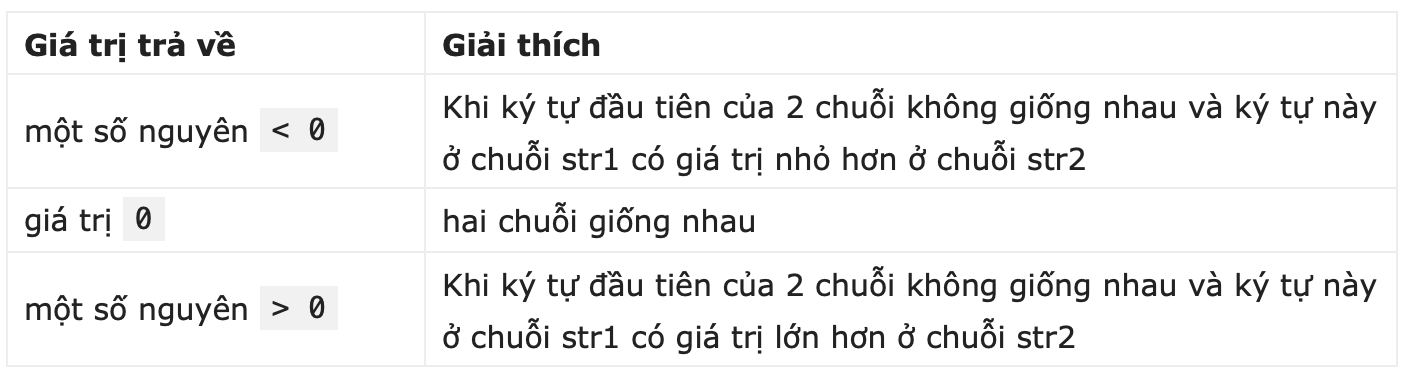
\includegraphics[scale = 0.57]{comparestring.png}
\end{center}
Đoạn code ví dụ sử dụng hàm strcmp:\\
\begin{lstlisting}
#include <stdio.h>
#include <string.h>
 
int main ()
{
  char key[] = "apple";
  char buffer[80];
  do {
     printf ("Hay doan loai qua toi thich? ");
     fflush (stdout);
     scanf ("%s",buffer);
  } while (strcmp (key,buffer) != 0);
  puts ("Ban doan dung roi!");
  return 0;
}
\end{lstlisting}
	\item Hàm \textbf{strcat} (hàm nối chuỗi):\\
Giúp ghép chuỗi nguồn phía sau và chuỗi đích, ví dụ thể hiện qua mã nguồn như sau:
\begin{lstlisting}
#include <stdio.h>
#include <string.h>
 
int main ()
{
  char str[80];
  strcpy (str,"Lap ");
  strcat (str,"trinh ");
  strcat (str,"khong ");
  strcat (str,"kho!");
  puts (str);
}
---------------------
KQ: Lap trinh khong kho!
\end{lstlisting}
	\item Hàm \textbf{strcpy} (Hàm copy chuỗi)\\ Hàm có tác dụng Copy giá trị của chuỗi nguồn và lưu vào chuỗi đích. Bạn cần dùng hàm này khi muốn gán giá trị của chuỗi này cho chuỗi khác thay vì sử dụng dấu "="
\begin{lstlisting}

#include <stdio.h>
#include <string.h>
 
int main ()
{
  char str1[]="Lap trinh khong kho!";
  char str2[40];
  char str3[40];
  strcpy (str2,str1);
  strcpy (str3,"Nguyen Van Hieu");
  printf ("str1: %s\nstr2: %s\nstr3: %s\n",str1,str2,str3);
  return 0;
}
------------
char * strcpy ( char * chuoi_dich, const char * chuoi_nguon);
\end{lstlisting}
	\item Hàm \textbf{strupr} (đưa chuỗi về dạng uppercase)
\begin{lstlisting}
	#include<stdio.h>
#include<string.h>
int main()
{
    char str[ ] = "Lap Trinh KHONG kho!";
    printf("%s\n",strupr (str));
}

\end{lstlisting}
	\item Hàm \textbf{strrev} (Hàm đảo ngược chuỗi)
\begin{lstlisting}
	#include <stdio.h>
#include <string.h>
 
int main()
{
    char name[30] = "Nguyen Van Hieu";
 
    printf("Truoc khi dao nguoc: %s\n", name);
 
    printf("Sau khi dao nguoc: %s", strrev(name));
 
    return 0;
}
\end{lstlisting}
\end{itemize}
\begin{center}
\subsection*{\textit{Nhập xuất chuỗi}} 	
\end{center}
\begin{itemize}
	\item Đối với chuỗi không chứa dấu trắng (dấu cách, dấu tab hay dấu xuống dòng), ta vẫn có thể nhập xuất chuỗi bình thường bằng lệnh scanf() và printf().  
\begin{lstlisting}
	#include <stdio.h>
	int main()
	{
    	char name[20];
    	printf("Enter name: ");
    	scanf("%s", name);
    	printf("Your name is %s.", name);
    	return 0;
	}
	-----
	Enter name: Tuan Anh Pham
	Your name is Tuan
\end{lstlisting}
như ta có thể thấy ở các câu lệnh trên, nó chỉ hiển thị chuỗi kí tự đầu trước phần có dấu cách, nếu bạn muốn xuất họ tên đầy đủ (có dấu cách, tab ...). Ta sẽ dùng \textbf{fgets()} để nhập và \textbf{puts()} để xuất chuỗi ra ngoài màn hình.
\begin{lstlisting}
#include <stdio.h>

int main(){
    char name[20];
    printf("Enter name: ");
    fgets(name, sizeof(name), stdin); 
    printf("Name: ");
    puts(name);    // display string
    return 0;
}
\end{lstlisting}
\end{itemize}
\section{Con Trỏ}
\begin{center}
	\subsection*{\textbf{\textit{Hiểu về con trỏ \& cách gọi, sử dụng}}}
\end{center}
\begin{itemize}
	\item Lý thuyết:\\
Con trỏ bản chất cũng là \textbf{biến} (có thể khai báo, khởi tạo, lưu trữ giá trị và có địa chỉ của riêng nó) nhưng giá trị của con trỏ lại biểu thị địa chỉ của các \textbf{biến} thông thường khác. Như đã đề cập, địa chỉ của biến khá quan trọng, nó giúp máy tính quản lý dữ liệu bằng các địa chỉ các ô trống chứa biến. Điều này dễ thấy qua tập lệnh sau:
\begin{lstlisting}
	int number;
	printf("\nNhap number = ");
	scanf("%d", &number);
	printf("\nnumber = %d", number);
\end{lstlisting}
Rõ ràng khi dùng hàm Scanf chúng ta cần truyền vào &number thế nhưng khi dùng hàm printf lại không cần dùng "\&" trước tên biến. Đơn giản vì nếu muốn nhập giá trị cho biến, hàm \textbf{scanf} cần biết địa chỉ của biến đó trong bộ nhớ đó rồi mới nhập giá trị vào.
	\item Khai báo, khởi tạo và sử dụng \footnote{Đặc biệt lưu ý khi khai báo con trỏ phải truyền ngay giá trị cho nó, nếu không giá trị của nó sẽ là giá trị rác, điều này sẽ cực kỳ nguy hiểm với chương trình của bạn}:\\
Một chút khác biệt so với khai báo biến bằng việc  thêm "\textbf{*}" trước tên biến để trình biên dịch biết ta đang khai báo con trỏ.
\begin{lstlisting}
	<type> * <name of variable>;
		-------------- Vi du ve khai bao bien con tro --------------
	int num = 5;
	int *p = &num;
\end{lstlisting}
\textbf{Lưu ý}: Sau lần khai báo đầu tiên truyền địa chỉ của biến vào con trỏ, việc gán một giá trị bất kì nào đó vào con trỏ sau đó sẽ được hiểu là tác dụng lên giá trị của biến mà con trỏ đang trỏ tới
\begin{lstlisting}
	#include <stdio.h>
	int main()
	{ 
  int value = 10;
    int *p = &value;
    printf("Gia tri cua bien: %d", value);
    printf("\nDia chi cua bien: %d", &value);
    printf("\nGia tri con tro: %d", p);
    printf("\nDia chi con tro: %d", &p);
    printf("\nGia tri bien noi con tro chi toi: %d", *p);
    printf("\n--- Cap nhat gia tri con tro ---");
    *p = 20;
    printf("\nGia tri cua bien khi cap nhat: %d", value);
    printf("\nGia tri bien ma con tro chi toi khi cap nhat: %d", *p);
    printf("\nDia chi con tro: %d\n", &p);
	}
------------
KQ:
Gia tri cua bien: 10
Dia chi cua bien: -272632436
Gia tri con tro: -272632436
Dia chi con tro: -272632448
Gia tri bien noi con tro chi toi: 10
--- Cap nhat gia tri con tro ---
Gia tri cua bien khi cap nhat: 20
Gia tri bien ma con tro chi toi khi cap nhat: 20
Dia chi con tro: -272632448
Program ended with exit code: 0
\end{lstlisting}
\end{itemize}

\begin{center}
	\subsection*{\textbf{\textit{Các mối liên hệ trong con trỏ}}}
\end{center}

\begin{itemize}
\item Liên hệ giữa con trỏ với \textbf{mảng}
Mảng như đã định nghĩa từ trước là một tập hợp tuần tự các phần tử có cùng kiểu dữ, và được lưu trong một dãy liên tục các bộ nhớ. Có thể hiểu rõ qua các câu lệnh sau:\\
\begin{lstlisting}

#include <stdio.h>
 
int main(){
    int arr[] = {1, 2, 3, 4, 5}; 
    printf("Dia chi cua mang arr = %d\n", &arr);
    printf("Gia chi cua mang arr = %d\n", arr);
    for(int i = 0; i < sizeof (arr) / sizeof (int); i++){
        printf("Dia chi cua arr[%d] = %d\n", i, &arr[i]);
    }
}
-----------
KQ:
Dia chi cua mang arr = 6487552
Gia chi cua mang arr = 6487552
Dia chi cua arr[0] = 6487552
Dia chi cua arr[1] = 6487556
Dia chi cua arr[2] = 6487560
Dia chi cua arr[3] = 6487564
Dia chi cua arr[4] = 6487568
\end{lstlisting}
Qua trên ta có vài nhận xét: 
\begin{itemize}
\item Các phần tử liên tiếp có địa chỉ cách nhau 4 giá trị (bởi vì 1 phần tử kiểu nguyên có kích thước 4 bytes). Điều đó củng cố cho định nghĩa các phần tử trong mảng xếp cạnh nhau.
\item Như đã đề cập là khi truyền mảng vào hàm thì mặc định là truyền theo tham chiếu. Và trong ví dụ này bạn thấy đó, địa chỉ và giá trị của biến mảng chính là địa chỉ của phần tử đầu tiên của mảng.
\item Như vậy, \&arr[0] tương đương \&arr và tương đương arr. Điều đó có được là do biến arr trỏ tới phần tử đầu tiên của mảng.
\end{itemize}

\item Liên hệ giữa con trỏ với \textbf{hàm}
Để dễ hiểu, tìm hiểu mối quan hệ giữa con trỏ với hàm thực ra là tìm hiểu về tham chiếu trong C và Truyền con trỏ vào hàm 
\begin{itemize}
\item {\large Tham chiếu}: \\
Xét qua ví dụ sau, có thể thấy hàm con không thay đổi giá trị của biến a và b trong hàm main(). Đó là bởi hàm của bạn đang truyền bởi tham trị – nghĩa là khi hàm swap() được gọi thì 2 tham số đó sẽ được hàm này sao chép sang 2 vùng nhớ mới, mọi thay đổi được thực hiện trên bản sao này.

\begin{lstlisting}
	#include <stdio.h>
 
	void swap(int a, int b){
    		printf("Ham con, truoc khi goi ham hoan vi, a = %d, b = %d\n", a , b);
    		int tmp = a;
    		a = b;
    		b = tmp;
    		printf("Ham con, sau khi goi ham hoan vi, a = %d, b = %d\n", a , b);
	}
 
	int main(){
    		int a = 5, b = 7;
    		printf("Ham main, truoc khi goi ham hoan vi, a = %d, b = %d\n", a , b);
    		swap(a, b);
    		printf("Ham main, sau khi goi ham hoan vi, a = %d, b = %d\n", a , b);
}
 ----------
 KQ:
	Ham main, truoc khi goi ham hoan vi, a = 5, b = 7
	Ham con, truoc khi goi ham hoan vi, a = 5, b = 7
	Ham con, sau khi goi ham hoan vi, a = 7, b = 5
	Ham main, sau khi goi ham hoan vi, a = 5, b = 7
\end{lstlisting}
Tương tự như bài toán này nhưng ta thử truyền tham chiếu bằng cách tham chiếu Và chứng minh cho việc khi ta có địa chỉ biến thì ta có thể thay đổi giá trị biến mà con trỏ đang truyền tới:
\begin{lstlisting}
#include <stdio.h>
 
void swap(int *a, int *b){
    printf("Ham con, truoc khi goi ham hoan vi, a = %d, b = %d\n", *a , *b);
    int tmp = *a; 
    *a = *b; 
    *b = tmp;
    printf("Ham con, sau khi goi ham hoan vi, a = %d, b = %d\n", *a , *b);
}
 
int main(){
    int a = 5, b = 7;
    printf("Ham main, truoc khi goi ham hoan vi, a = %d, b = %d\n", a , b);
    swap(&a, &b);
    printf("Ham main, sau khi goi ham hoan vi, a = %d, b = %d\n", a , b);
}
--------
KQ:
Ham main, truoc khi goi ham hoan vi, a = 5, b = 7
Ham con, truoc khi goi ham hoan vi, a = 5, b = 7
Ham con, sau khi goi ham hoan vi, a = 7, b = 5
Ham main, sau khi goi ham hoan vi, a = 7, b = 5 
\end{lstlisting}

\item {\large Truyền con trỏ vào hàm}\\
Chúng ta đã quen với truyền giá trị vào hàm (truyền tham trị) ta cũng vừa làm quen với truyền tham chiếu qua đoạn code ở trên, qua phần này chúng ta sẽ hiểu rõ hơn về truyền con trỏ vào hàm trong C:
\begin{lstlisting}
#include <stdio.h>
 
void addOne(int *ptr)
{
    (*ptr)++;
}
int main()
{
    int *p, i = 10;
    p = &i;
    addOne(p);
    printf("%d", *p); // Dap an: 11
    return 0;
}
\end{lstlisting} 
\end{itemize}

\begin{center}
	\subsection*{\textbf{\textit{Cấp phát bộ nhớ cho con trỏ}}}
\end{center}
Một phần quan trọng khi làm quen và sử dụng con trỏ là cấp phát bộ nhớ động và giải phóng bộ nhớ bằng việc sử dụng các hàm malloc(), calloc(), free() và realloc() trong C
\begin{itemize}
\item Tại sao cần cấp phát bộ nhớ động, những định nghĩa ...\\
Nói đến con trỏ không thể không nhắc tới các định nghĩa về \textbf{cấp phát bộ nhớ động} và \textbf{giải phóng bộ nhớ}. Chúng ta sẽ làm rõ vấn đề này về việc cấp phát bộ nhớ động sử dụng các hàm \textbf{malloc(), calloc(), free() và realloc()}\\
Quay trở lại mảng, như ta đã biết và thường làm trước đó, ta thường chỉ định rõ kích thước tối đa của \textbf{mảng} và sau khi khai báo ta không thể thay đổi kích thước của mảng được nữa $\Rightarrow$ Cấp phát tĩnh.\\
Điều đó nảy sinh ra vấn đề là có thể kích thước giới hạn định sẵn đó không đủ dùng, để giải quyết vấn đề ta có cấp phát bộ nhớ theo cách thủ công trong thời gian chạy chương trình.
\item Cấp phát và sử dụng bộ nhớ qua các hàm\\
\begin{itemize}
\item Sử dụng hàm malloc (memory allocation)\\
Hàm malloc() thực hiện cấp phát bộ nhớ bằng cách chỉ định số byte cần cấp và trả về kiểu \textbf{void} giúp ta có thể ép kiểu thành bất cứ kiểu dữ liệu nào. Cú pháp: 
\begin{lstlisting}
ptr = (castType*) malloc(size);
----- Vi Du -----
ptr = (int*) malloc(100 * sizeof(int));
\end{lstlisting}	
Ở ví dụ trên, ta thực hiện việc lưu trữ 100 số nguyên. Với \textbf{sizeof (int)} là 4, khi đó lệnh malloc() thực hiện cấp phát 400 bytes. Khi đó, con trỏ "ptr" có giá trị là địa chỉ của byte dữ liệu đầu tiên trong khôí bộ nhớ.
\item Sử dụng hàm calloc (contiguous allocation)\\
Đối với hàm malloc() khi cấp phát bộ nhớ thì vùng nhớ cấp phát đó không được khởi tạo giá trị ban đầu. Trong khi đó, hàm calloc() thực hiện cấp phát bộ nhớ và khởi tạo tất cả các ô nhớ có giá trị bằng 0/
\begin{lstlisting}
ptr = (castType*)calloc(n, size);
------ Vi du ------
ptr = (int*) calloc(100, sizeof(int));
\end{lstlisting}
Trong ví dụ trên, hàm calloc() thực hiện cấp phát 100 ô nhớ liên tiếp và mỗi ô nhớ có kích thước là số byte của kiểu int. Hàm này cũng trả về con trỏ chứa giá trị là địa chỉ của byte đầu tiên trong khối bộ nhớ vừa cấp phát.
\item Sử dụng hàm free()\\
Việc cấp phát bộ nhớ động trong C dù sử dụng malloc() hay calloc() thì chúng cũng đều không thể tự giải phóng bộ nhớ. Bạn cần sử dụng hàm free() để \textbf{giải phóng vùng nhớ} không dùng tới để tối ưu dụng lượng trống hệ thống .
\begin{lstlisting}
free(ptr);
\end{lstlisting}
Lệnh này sẽ giải phóng vùng nhớ mà con trỏ ptr đã được cấp phát. Giải phóng ở đây có nghĩa là trả lại vùng nhớ đó cho hệ điều hành và hệ điều hành có thể sử dụng vùng nhớ đó vào việc khác nếu cần.\\


Nếu bạn không giải phóng nó thì nó sẽ tồn tại cho tới khi chương trình kết thúc. Điều này sẽ rất nguy hiểm nếu chương trình của bạn liên tục cấp phát các vùng nhớ mới và sẽ gây ra hiện tượng tràn bộ nhớ mà mình đã nhắc tới ở trên. Thử code này xem sao (bảo đảm là máy bạn sẽ bị treo và chỉ còn cách ấn nút nguồn thôi, bạn có thể để cấp phát size nhỏ hơn và theo dõi thay đổi qua Task Manager)
\item Sử dụng hàm malloc() và free():\\
Trong ví dụ dưới đây, chúng ta sẽ sử dụng hàm \textbf{malloc()} để cấp phát động n * sizeof int byte và sử dụng xong sẽ dùng free() để giải phóng.
\begin{lstlisting}
#include <stdio.h>
#include <stdlib.h>
 
int main()
{
    int n, i, *ptr, sum = 0;
    printf("Nhap so luong phan tu: ");
    scanf("%d", &n);
    ptr = (int *)malloc(n * sizeof(int));
 
    if (ptr == NULL)
    {
        printf("Co loi! khong the cap phat bo nho.");
        exit(0);
    }
    printf("Nhap cac gia tri: ");
    for (i = 0; i < n; ++i)
    {
        scanf("%d", ptr + i);
        sum += *(ptr + i);
    }
    printf("Tong = %d", sum);
 
    // Giai phong bo nho con tro
    free(ptr);
    return 0;
}
\end{lstlisting}
\item Sử dụng hàm \textbf{calloc()} và \textbf{free()}\\
Trong ví dụ này, chúng ta sẽ dùng calloc() để cấp phát n ô nhớ liên tiếp và mỗi ô nhớ có kích thước là sizeof int. Lưu ý là hàm calloc() sẽ chậm hơn malloc() một chút do nó phải thêm bước khởi tạo các ô nhớ có giá trị bằng 0.
\begin{lstlisting} 
#include <stdio.h>
#include <stdlib.h>
 
int main()
{
    int n, i, *ptr, sum = 0;
    printf("Nhap so luong phan tu: ");
    scanf("%d", &n);
    ptr = (int *)calloc(n, sizeof(int));
 
    if (ptr == NULL)
    {
        printf("Co loi! khong the cap phat bo nho.");
        exit(0);
    }
    printf("Nhap cac gia tri: ");
    for (i = 0; i < n; ++i)
    {
        scanf("%d", ptr + i);
        sum += *(ptr + i);
    }
    printf("Tong = %d", sum);
 
    free(ptr);
    return 0;
}
\end{lstlisting}
\item Sử dụng hàm \textbf{realloc()};
Nếu việc cấp phát bộ nhớ động không đủ hoặc cần nhiều hơn mức đã cấp phát, bạn có thể thay đổi kích thước của bộ nhớ đã được cấp phát trước đó bằng cách sử dụng hàm realloc().\\
Chúng ta thực hiện cấp phát vùng nhớ mới cho con trỏ ptr, vùng nhớ mới sẽ có kích thước là n bytes qua cú pháp sau:
\begin{lstlisting}
ptr = realloc(ptr, n);
\end{lstlisting}
Một ví dụ về việc sử dụng hàm realloc() để tái phân lại bộ nhớ :
\begin{lstlisting}
#include <stdio.h>
#include <stdlib.h>
int main()
{
    int *ptr, i , n1, n2;
    printf("Nhap so luong phan tu: ");
    scanf("%d", &n1);
    ptr = (int*) malloc(n1 * sizeof(int));
    printf("Dia chi cua vung nho vua cap phat: %u", ptr);
    
    printf("\nNhap lai so luong phan tu: ");
    scanf("%d", &n2);
    // phan bo lai vung nho
    ptr = (int*) realloc(ptr, n2 * sizeof(int));
    printf("Dia chi cua vung nho duoc cap phat lai: %u", ptr);
    // giai phong 
    free(ptr);
    return 0;
}
\end{lstlisting}
\end{itemize}
\end{itemize}
\section{Kiểu Struct trong C}
\begin{center}
	\subsection*{\textbf{\textit{Hiểu về Struct \& cách gọi, sử dụng}}}
\end{center}
\begin{itemize}
\item {\large Tổng quan:}\\
Như được làm quen với mảng trước đó, chúng cho phép bạn lưu trữ các giá trị của các bién có cùng kiểu dữ liệu. Làm quen với kiểu \textbf{Struct} lại là một loại tổ chức dữ liệu khác trong lập trình đó là cho phép kết hợp các kiểu dữ liệu khác kiểu nhau (hơi ngược với kiểu lưu trữ mảng).\\

\textbf{Struct} thực sự hoạt động thế nào ? Một cách dễ hình dung, Struct tổ chức dữ liệu bạn dưới dạng bản ghi. Nghĩa là bạn giả sử muốn lưu trữ giá trị của một quyển sách trong thư viện của bạn. Bạn sẽ quan tâm đến những yếu tố sau của cuốn sách và đó là cách Struct giúp bạn quản lý và sử dụng:
\begin{itemize}
\item Tiêu đề
\item Tác giả
\item Chủ đề
\item Book ID
\end{itemize}

\item {\large Cú pháp định nghĩa kiểu :}\\
Trước khi chúng ta có thể khai báo biến với struct, bạn cần định nghĩa nó – Đó cũng là lý do tại sao struct được gọi là kiểu dữ liệu người dùng định nghĩa.\\
Khi nào ta cần tự định nghĩa kiểu cấu trúc đó là khi cần lưu trữ một đối tượng có nhiều thược tính. Ví dụ, đối tượng SinhVien có các thuộc tính (MSV, họ, tên, giới tính, quê quán,…). Khi đó chúng ta dùng struct để quản lý chương trình. Cú pháp định nghĩa :
\begin{lstlisting}
struct structureName 
{
    dataType member1;
    dataType member2;
    ...
};
---------- Vi du ----------
struct SinhVien {
    int maSV;
    char ho[20];
    char ten[20];
    bool gioiTinh;
    char queQuan[100];
};
\end{lstlisting}

\item {\large Khai báo biến kiểu \textbf{Struct}}:\\
Việc khai báo biến với \textbf{struct} cũng giống như cách khai báo biến thông thường, trong đó kiểu dữ liệu là kiểu struct trong C mà bạn vừa định nghĩa.
\begin{lstlisting}
struct SinhVien
{
    int maSV;
    char ho[20];
    char ten[20];
    bool gioiTinh;
    char queQuan[100];
};
 
int main(){
	//khai bao 2 bien sv1 va sv2 co kieu SinhVien
    SinhVien sv1, sv2;
 
    // Nen them tu khoa Struct o tren dau
    // De phan biet du lieu tu dinh nghia 
    struct SinhVien sv3, sv4;
 
    // Khai bao mang
    struct SinhVien sv[100];
}
\end{lstlisting}
\item {\large Truy xuất các thuộc tính cùa kiểu \textbf{Struct}}:\\
Ta sử dụng 2 toán tử để truy xuất tới các biến thành viên của kiểu 
\begin{itemize}
\item Sử dụng "." $\Rightarrow$ Toán tử truy xuất tới thành viên khi khai báo biến bình thường 
\item Sử dụng "->" $\Rightarrow$ Toán tử truy xuất tới thành viên khi biến là con trỏ.\\
Giả sử bạn muốn truy suất \textbf{"gioiTinh"} của đối tượng Sinh Viên thì làm như sau:
\begin{lstlisting}
SinhVien sv;
// to do
printf("Gioi tinh: %s", sv.gioiTinh);
\end{lstlisting} 
\end{itemize}
\item {\large Từ khoá \textbf{typedef}}:\\
Bạn có thể sử dụng từ khóa \textbf{typedef} để tạo ra một tên thay thế cho kiểu dữ liệu đã có. Nó thường được sử dụng kiểu \textbf{struct} để đơn giản hóa cú pháp khai báo biến. Nhưng nó cũng có thể sử dụng với các kiểu dữ liệu nguyên thủy nhé.
\begin{lstlisting}
struct Distance{
    int feet;
    float inch;
};
 
int main() {
    structure Distance d1, d2;
}
 ---- Tuong Duong ---- 
 typedef struct SinhVien{
    int feet;
    float inch;
} distances;
 
int main() {
    distances d1, d2;
}
---- Hoac ---- 
struct PhanSo{
    int tu;
    int mau;
};
typedef struct PhanSo PS;
\end{lstlisting}
\item {\large Cấu trúc \textbf{Struct} lồng nhau}:\\
Giả sử bạn muốn xây dựng kiểu dữ liệu để lưu trữ đối tượng Tam giác, khi đó chúng ta có thể xây dựng \textbf{struct} mô tả tọa độ của 1 điểm, khi đó đối tượng tam giác sẽ là 3 đối tượng điểm. Cụ thể:
\begin{lstlisting}
struct Point{
    int x; // Hoanh do
    int y; // Tung do
};
 
struct Triangle{
    Point a; //dinh thu nhat
    Point b; //dinh thu hai
    Point c; //dinh thu ba
}
 
int main(){
    Triangle tg;
    
    // truy xuat hoanh do cua diem thu nhat
    tg.a.x = 5;
}
\end{lstlisting}

\end{itemize}

\end{document}
